% Created by tikzDevice version 0.10.1 on 2017-03-15 16:22:39
% !TEX encoding = UTF-8 Unicode
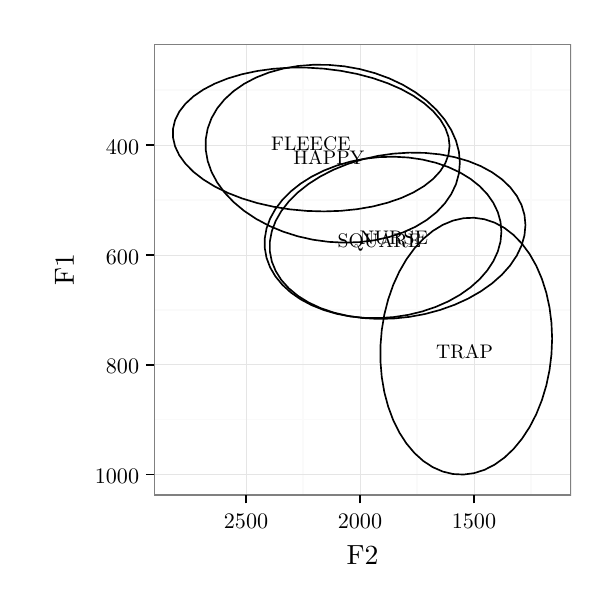
\begin{tikzpicture}[x=1pt,y=1pt]
\definecolor{fillColor}{RGB}{255,255,255}
\path[use as bounding box,fill=fillColor,fill opacity=0.00] (0,0) rectangle (202.36,202.36);
\begin{scope}
\path[clip] (  0.00,  0.00) rectangle (202.36,202.36);
\definecolor{drawColor}{RGB}{255,255,255}
\definecolor{fillColor}{RGB}{255,255,255}

\path[draw=drawColor,line width= 0.6pt,line join=round,line cap=round,fill=fillColor] (  0.00,  0.00) rectangle (202.36,202.36);
\end{scope}
\begin{scope}
\path[clip] ( 45.67, 33.48) rectangle (196.36,196.36);
\definecolor{fillColor}{RGB}{255,255,255}

\path[fill=fillColor] ( 45.67, 33.48) rectangle (196.36,196.36);
\definecolor{drawColor}{gray}{0.98}

\path[draw=drawColor,line width= 0.6pt,line join=round] ( 45.67,179.73) --
	(196.36,179.73);

\path[draw=drawColor,line width= 0.6pt,line join=round] ( 45.67,140.06) --
	(196.36,140.06);

\path[draw=drawColor,line width= 0.6pt,line join=round] ( 45.67,100.39) --
	(196.36,100.39);

\path[draw=drawColor,line width= 0.6pt,line join=round] ( 45.67, 60.72) --
	(196.36, 60.72);

\path[draw=drawColor,line width= 0.6pt,line join=round] (181.85, 33.48) --
	(181.85,196.36);

\path[draw=drawColor,line width= 0.6pt,line join=round] (140.67, 33.48) --
	(140.67,196.36);

\path[draw=drawColor,line width= 0.6pt,line join=round] ( 99.49, 33.48) --
	( 99.49,196.36);
\definecolor{drawColor}{gray}{0.90}

\path[draw=drawColor,line width= 0.2pt,line join=round] ( 45.67,159.89) --
	(196.36,159.89);

\path[draw=drawColor,line width= 0.2pt,line join=round] ( 45.67,120.22) --
	(196.36,120.22);

\path[draw=drawColor,line width= 0.2pt,line join=round] ( 45.67, 80.55) --
	(196.36, 80.55);

\path[draw=drawColor,line width= 0.2pt,line join=round] ( 45.67, 40.88) --
	(196.36, 40.88);

\path[draw=drawColor,line width= 0.2pt,line join=round] (161.26, 33.48) --
	(161.26,196.36);

\path[draw=drawColor,line width= 0.2pt,line join=round] (120.08, 33.48) --
	(120.08,196.36);

\path[draw=drawColor,line width= 0.2pt,line join=round] ( 78.90, 33.48) --
	( 78.90,196.36);
\definecolor{drawColor}{RGB}{0,0,0}

\node[text=drawColor,anchor=base,inner sep=0pt, outer sep=0pt, scale=  0.71] at (102.35,157.97) {FLEECE};

\node[text=drawColor,anchor=base,inner sep=0pt, outer sep=0pt, scale=  0.71] at (108.87,152.81) {HAPPY};

\node[text=drawColor,anchor=base,inner sep=0pt, outer sep=0pt, scale=  0.71] at (132.29,123.92) {NURSE};

\node[text=drawColor,anchor=base,inner sep=0pt, outer sep=0pt, scale=  0.71] at (127.12,123.10) {SQUARE};

\node[text=drawColor,anchor=base,inner sep=0pt, outer sep=0pt, scale=  0.71] at (157.86, 82.93) {TRAP};

\path[draw=drawColor,line width= 0.6pt,line join=round] (152.45,159.68) --
	(152.07,162.88) --
	(150.94,166.06) --
	(149.07,169.19) --
	(146.50,172.20) --
	(143.26,175.06) --
	(139.40,177.72) --
	(134.98,180.15) --
	(130.06,182.29) --
	(124.73,184.13) --
	(119.06,185.63) --
	(113.14,186.77) --
	(107.05,187.54) --
	(100.90,187.92) --
	( 94.76,187.91) --
	( 88.75,187.50) --
	( 82.94,186.70) --
	( 77.43,185.53) --
	( 72.30,184.01) --
	( 67.62,182.14) --
	( 63.47,179.98) --
	( 59.91,177.54) --
	( 57.00,174.86) --
	( 54.77,171.99) --
	( 53.27,168.96) --
	( 52.52,165.83) --
	( 52.52,162.64) --
	( 53.27,159.44) --
	( 54.77,156.28) --
	( 57.00,153.21) --
	( 59.91,150.26) --
	( 63.47,147.50) --
	( 67.62,144.95) --
	( 72.30,142.66) --
	( 77.43,140.67) --
	( 82.94,138.99) --
	( 88.75,137.67) --
	( 94.76,136.71) --
	(100.90,136.14) --
	(107.05,135.96) --
	(113.14,136.17) --
	(119.06,136.77) --
	(124.73,137.75) --
	(130.06,139.11) --
	(134.98,140.80) --
	(139.40,142.82) --
	(143.26,145.13) --
	(146.50,147.69) --
	(149.07,150.47) --
	(150.94,153.43) --
	(152.07,156.51) --
	(152.45,159.68);

\path[draw=drawColor,line width= 0.6pt,line join=round] (156.17,153.56) --
	(155.83,157.52) --
	(154.79,161.47) --
	(153.07,165.34) --
	(150.71,169.09) --
	(147.73,172.65) --
	(144.18,175.97) --
	(140.12,179.00) --
	(135.60,181.70) --
	(130.70,184.02) --
	(125.49,185.92) --
	(120.05,187.39) --
	(114.46,188.39) --
	(108.80,188.91) --
	(103.17,188.95) --
	( 97.64,188.50) --
	( 92.31,187.57) --
	( 87.24,186.18) --
	( 82.53,184.34) --
	( 78.23,182.08) --
	( 74.42,179.44) --
	( 71.15,176.46) --
	( 68.47,173.18) --
	( 66.43,169.65) --
	( 65.05,165.93) --
	( 64.35,162.07) --
	( 64.35,158.13) --
	( 65.05,154.17) --
	( 66.43,150.25) --
	( 68.47,146.44) --
	( 71.15,142.77) --
	( 74.42,139.33) --
	( 78.23,136.14) --
	( 82.53,133.28) --
	( 87.24,130.76) --
	( 92.31,128.65) --
	( 97.64,126.96) --
	(103.17,125.72) --
	(108.80,124.96) --
	(114.46,124.68) --
	(120.05,124.88) --
	(125.49,125.57) --
	(130.70,126.74) --
	(135.60,128.36) --
	(140.12,130.41) --
	(144.18,132.86) --
	(147.73,135.68) --
	(150.71,138.82) --
	(153.07,142.23) --
	(154.79,145.86) --
	(155.83,149.66) --
	(156.17,153.56);

\path[draw=drawColor,line width= 0.6pt,line join=round] (179.87,131.05) --
	(179.52,134.68) --
	(178.48,138.20) --
	(176.75,141.55) --
	(174.37,144.69) --
	(171.38,147.55) --
	(167.81,150.11) --
	(163.72,152.33) --
	(159.18,154.16) --
	(154.25,155.58) --
	(149.01,156.57) --
	(143.54,157.11) --
	(137.92,157.20) --
	(132.23,156.84) --
	(126.56,156.03) --
	(121.00,154.77) --
	(115.64,153.10) --
	(110.54,151.04) --
	(105.80,148.62) --
	(101.48,145.87) --
	( 97.64,142.83) --
	( 94.36,139.56) --
	( 91.66,136.10) --
	( 89.61,132.51) --
	( 88.22,128.83) --
	( 87.52,125.13) --
	( 87.52,121.46) --
	( 88.22,117.88) --
	( 89.61,114.44) --
	( 91.66,111.19) --
	( 94.36,108.18) --
	( 97.64,105.46) --
	(101.48,103.07) --
	(105.80,101.05) --
	(110.54, 99.42) --
	(115.64, 98.21) --
	(121.00, 97.44) --
	(126.56, 97.12) --
	(132.23, 97.26) --
	(137.92, 97.85) --
	(143.54, 98.88) --
	(149.01,100.35) --
	(154.25,102.22) --
	(159.18,104.46) --
	(163.72,107.06) --
	(167.81,109.95) --
	(171.38,113.11) --
	(174.37,116.48) --
	(176.75,120.02) --
	(178.48,123.66) --
	(179.52,127.35) --
	(179.87,131.05);

\path[draw=drawColor,line width= 0.6pt,line join=round] (171.18,128.67) --
	(170.86,132.23) --
	(169.89,135.70) --
	(168.29,139.03) --
	(166.09,142.18) --
	(163.32,145.09) --
	(160.01,147.72) --
	(156.23,150.03) --
	(152.03,151.98) --
	(147.46,153.55) --
	(142.61,154.71) --
	(137.54,155.44) --
	(132.34,155.73) --
	(127.07,155.58) --
	(121.83,155.00) --
	(116.68,153.98) --
	(111.71,152.54) --
	(106.99,150.71) --
	(102.60,148.52) --
	( 98.60,145.99) --
	( 95.05,143.17) --
	( 92.01,140.10) --
	( 89.51,136.82) --
	( 87.61,133.38) --
	( 86.32,129.85) --
	( 85.68,126.26) --
	( 85.68,122.68) --
	( 86.32,119.15) --
	( 87.61,115.74) --
	( 89.51,112.50) --
	( 92.01,109.46) --
	( 95.05,106.69) --
	( 98.60,104.21) --
	(102.60,102.08) --
	(106.99,100.32) --
	(111.71, 98.95) --
	(116.68, 98.00) --
	(121.83, 97.49) --
	(127.07, 97.42) --
	(132.34, 97.79) --
	(137.54, 98.59) --
	(142.61, 99.82) --
	(147.46,101.46) --
	(152.03,103.47) --
	(156.23,105.84) --
	(160.01,108.51) --
	(163.32,111.47) --
	(166.09,114.65) --
	(168.29,118.01) --
	(169.89,121.50) --
	(170.86,125.07) --
	(171.18,128.67);

\path[draw=drawColor,line width= 0.6pt,line join=round] (189.51, 90.01) --
	(189.27, 95.69) --
	(188.57,101.23) --
	(187.41,106.57) --
	(185.81,111.61) --
	(183.80,116.28) --
	(181.40,120.52) --
	(178.66,124.25) --
	(175.61,127.42) --
	(172.30,129.98) --
	(168.78,131.89) --
	(165.11,133.13) --
	(161.33,133.67) --
	(157.51,133.51) --
	(153.70,132.65) --
	(149.97,131.10) --
	(146.37,128.89) --
	(142.94,126.04) --
	(139.76,122.61) --
	(136.86,118.65) --
	(134.28,114.20) --
	(132.07,109.35) --
	(130.27,104.17) --
	(128.88, 98.73) --
	(127.95, 93.11) --
	(127.48, 87.41) --
	(127.48, 81.70) --
	(127.95, 76.08) --
	(128.88, 70.63) --
	(130.27, 65.43) --
	(132.07, 60.57) --
	(134.28, 56.10) --
	(136.86, 52.11) --
	(139.76, 48.66) --
	(142.94, 45.79) --
	(146.37, 43.55) --
	(149.97, 41.97) --
	(153.70, 41.07) --
	(157.51, 40.88) --
	(161.33, 41.39) --
	(165.11, 42.60) --
	(168.78, 44.49) --
	(172.30, 47.02) --
	(175.61, 50.16) --
	(178.66, 53.87) --
	(181.40, 58.08) --
	(183.80, 62.74) --
	(185.81, 67.77) --
	(187.41, 73.09) --
	(188.57, 78.63) --
	(189.27, 84.30) --
	(189.51, 90.01);
\definecolor{drawColor}{gray}{0.50}

\path[draw=drawColor,line width= 0.6pt,line join=round,line cap=round] ( 45.67, 33.48) rectangle (196.36,196.36);
\end{scope}
\begin{scope}
\path[clip] (  0.00,  0.00) rectangle (202.36,202.36);
\definecolor{drawColor}{RGB}{0,0,0}

\node[text=drawColor,anchor=base east,inner sep=0pt, outer sep=0pt, scale=  0.80] at ( 40.27,156.59) {400};

\node[text=drawColor,anchor=base east,inner sep=0pt, outer sep=0pt, scale=  0.80] at ( 40.27,116.92) {600};

\node[text=drawColor,anchor=base east,inner sep=0pt, outer sep=0pt, scale=  0.80] at ( 40.27, 77.25) {800};

\node[text=drawColor,anchor=base east,inner sep=0pt, outer sep=0pt, scale=  0.80] at ( 40.27, 37.58) {1000};
\end{scope}
\begin{scope}
\path[clip] (  0.00,  0.00) rectangle (202.36,202.36);
\definecolor{drawColor}{RGB}{0,0,0}

\path[draw=drawColor,line width= 0.6pt,line join=round] ( 42.67,159.89) --
	( 45.67,159.89);

\path[draw=drawColor,line width= 0.6pt,line join=round] ( 42.67,120.22) --
	( 45.67,120.22);

\path[draw=drawColor,line width= 0.6pt,line join=round] ( 42.67, 80.55) --
	( 45.67, 80.55);

\path[draw=drawColor,line width= 0.6pt,line join=round] ( 42.67, 40.88) --
	( 45.67, 40.88);
\end{scope}
\begin{scope}
\path[clip] (  0.00,  0.00) rectangle (202.36,202.36);
\definecolor{drawColor}{RGB}{0,0,0}

\path[draw=drawColor,line width= 0.6pt,line join=round] (161.26, 30.48) --
	(161.26, 33.48);

\path[draw=drawColor,line width= 0.6pt,line join=round] (120.08, 30.48) --
	(120.08, 33.48);

\path[draw=drawColor,line width= 0.6pt,line join=round] ( 78.90, 30.48) --
	( 78.90, 33.48);
\end{scope}
\begin{scope}
\path[clip] (  0.00,  0.00) rectangle (202.36,202.36);
\definecolor{drawColor}{RGB}{0,0,0}

\node[text=drawColor,anchor=base,inner sep=0pt, outer sep=0pt, scale=  0.80] at (161.26, 21.47) {1500};

\node[text=drawColor,anchor=base,inner sep=0pt, outer sep=0pt, scale=  0.80] at (120.08, 21.47) {2000};

\node[text=drawColor,anchor=base,inner sep=0pt, outer sep=0pt, scale=  0.80] at ( 78.90, 21.47) {2500};
\end{scope}
\begin{scope}
\path[clip] (  0.00,  0.00) rectangle (202.36,202.36);
\definecolor{drawColor}{RGB}{0,0,0}

\node[text=drawColor,anchor=base,inner sep=0pt, outer sep=0pt, scale=  1.00] at (121.01,  8.40) {F2};
\end{scope}
\begin{scope}
\path[clip] (  0.00,  0.00) rectangle (202.36,202.36);
\definecolor{drawColor}{RGB}{0,0,0}

\node[text=drawColor,rotate= 90.00,anchor=base,inner sep=0pt, outer sep=0pt, scale=  1.00] at ( 16.67,114.92) {F1};
\end{scope}
\end{tikzpicture}
